% Options for packages loaded elsewhere
\PassOptionsToPackage{unicode}{hyperref}
\PassOptionsToPackage{hyphens}{url}
\PassOptionsToPackage{dvipsnames,svgnames,x11names}{xcolor}
%
\documentclass[
]{article}

\usepackage{amsmath,amssymb}
\usepackage{iftex}
\ifPDFTeX
  \usepackage[T1]{fontenc}
  \usepackage[utf8]{inputenc}
  \usepackage{textcomp} % provide euro and other symbols
\else % if luatex or xetex
  \usepackage{unicode-math}
  \defaultfontfeatures{Scale=MatchLowercase}
  \defaultfontfeatures[\rmfamily]{Ligatures=TeX,Scale=1}
\fi
\usepackage{lmodern}
\ifPDFTeX\else  
    % xetex/luatex font selection
    \setmainfont[]{Latin Modern Roman}
  \setmathfont[]{Latin Modern Math}
\fi
% Use upquote if available, for straight quotes in verbatim environments
\IfFileExists{upquote.sty}{\usepackage{upquote}}{}
\IfFileExists{microtype.sty}{% use microtype if available
  \usepackage[]{microtype}
  \UseMicrotypeSet[protrusion]{basicmath} % disable protrusion for tt fonts
}{}
\makeatletter
\@ifundefined{KOMAClassName}{% if non-KOMA class
  \IfFileExists{parskip.sty}{%
    \usepackage{parskip}
  }{% else
    \setlength{\parindent}{0pt}
    \setlength{\parskip}{6pt plus 2pt minus 1pt}}
}{% if KOMA class
  \KOMAoptions{parskip=half}}
\makeatother
\usepackage{xcolor}
\setlength{\emergencystretch}{3em} % prevent overfull lines
\setcounter{secnumdepth}{5}
% Make \paragraph and \subparagraph free-standing
\makeatletter
\ifx\paragraph\undefined\else
  \let\oldparagraph\paragraph
  \renewcommand{\paragraph}{
    \@ifstar
      \xxxParagraphStar
      \xxxParagraphNoStar
  }
  \newcommand{\xxxParagraphStar}[1]{\oldparagraph*{#1}\mbox{}}
  \newcommand{\xxxParagraphNoStar}[1]{\oldparagraph{#1}\mbox{}}
\fi
\ifx\subparagraph\undefined\else
  \let\oldsubparagraph\subparagraph
  \renewcommand{\subparagraph}{
    \@ifstar
      \xxxSubParagraphStar
      \xxxSubParagraphNoStar
  }
  \newcommand{\xxxSubParagraphStar}[1]{\oldsubparagraph*{#1}\mbox{}}
  \newcommand{\xxxSubParagraphNoStar}[1]{\oldsubparagraph{#1}\mbox{}}
\fi
\makeatother


\providecommand{\tightlist}{%
  \setlength{\itemsep}{0pt}\setlength{\parskip}{0pt}}\usepackage{longtable,booktabs,array}
\usepackage{calc} % for calculating minipage widths
% Correct order of tables after \paragraph or \subparagraph
\usepackage{etoolbox}
\makeatletter
\patchcmd\longtable{\par}{\if@noskipsec\mbox{}\fi\par}{}{}
\makeatother
% Allow footnotes in longtable head/foot
\IfFileExists{footnotehyper.sty}{\usepackage{footnotehyper}}{\usepackage{footnote}}
\makesavenoteenv{longtable}
\usepackage{graphicx}
\makeatletter
\def\maxwidth{\ifdim\Gin@nat@width>\linewidth\linewidth\else\Gin@nat@width\fi}
\def\maxheight{\ifdim\Gin@nat@height>\textheight\textheight\else\Gin@nat@height\fi}
\makeatother
% Scale images if necessary, so that they will not overflow the page
% margins by default, and it is still possible to overwrite the defaults
% using explicit options in \includegraphics[width, height, ...]{}
\setkeys{Gin}{width=\maxwidth,height=\maxheight,keepaspectratio}
% Set default figure placement to htbp
\makeatletter
\def\fps@figure{htbp}
\makeatother

\usepackage{arxiv}
\usepackage{orcidlink}
\usepackage{amsmath}
\usepackage[T1]{fontenc}
\makeatletter
\@ifpackageloaded{caption}{}{\usepackage{caption}}
\AtBeginDocument{%
\ifdefined\contentsname
  \renewcommand*\contentsname{Table of contents}
\else
  \newcommand\contentsname{Table of contents}
\fi
\ifdefined\listfigurename
  \renewcommand*\listfigurename{List of Figures}
\else
  \newcommand\listfigurename{List of Figures}
\fi
\ifdefined\listtablename
  \renewcommand*\listtablename{List of Tables}
\else
  \newcommand\listtablename{List of Tables}
\fi
\ifdefined\figurename
  \renewcommand*\figurename{Figure}
\else
  \newcommand\figurename{Figure}
\fi
\ifdefined\tablename
  \renewcommand*\tablename{Table}
\else
  \newcommand\tablename{Table}
\fi
}
\@ifpackageloaded{float}{}{\usepackage{float}}
\floatstyle{ruled}
\@ifundefined{c@chapter}{\newfloat{codelisting}{h}{lop}}{\newfloat{codelisting}{h}{lop}[chapter]}
\floatname{codelisting}{Listing}
\newcommand*\listoflistings{\listof{codelisting}{List of Listings}}
\makeatother
\makeatletter
\makeatother
\makeatletter
\@ifpackageloaded{caption}{}{\usepackage{caption}}
\@ifpackageloaded{subcaption}{}{\usepackage{subcaption}}
\makeatother
\makeatletter
\@ifpackageloaded{sidenotes}{}{\usepackage{sidenotes}}
\@ifpackageloaded{marginnote}{}{\usepackage{marginnote}}
\makeatother

\ifLuaTeX
  \usepackage{selnolig}  % disable illegal ligatures
\fi
\usepackage{bookmark}

\IfFileExists{xurl.sty}{\usepackage{xurl}}{} % add URL line breaks if available
\urlstyle{same} % disable monospaced font for URLs
\hypersetup{
  pdftitle={Experiment Result: Two Phase Flow},
  pdfauthor={Jayjay, Tuna, Jason, Richard},
  colorlinks=true,
  linkcolor={blue},
  filecolor={Maroon},
  citecolor={Blue},
  urlcolor={Blue},
  pdfcreator={LaTeX via pandoc}}


\renewcommand{\today}{2024-09-30}
\newcommand{\runninghead}{A Preprint }
\renewcommand{\runninghead}{A Preprint }
\title{Experiment Result: Two Phase Flow}
\def\asep{\\\\\\ } % default: all authors on same column
\author{\textbf{Jayjay, Tuna, Jason, Richard}\\}
\date{2024-09-30}
\begin{document}
\maketitle


We now evaluate surrogate models in two different criteria, forward
simulation and inverse problem.

\section{Pipeline}\label{pipeline}

\begin{itemize}
\tightlist
\item
  \textbf{FNO-NF.jl}: create two-phase flow dataset, eigenvector of FIM,
  and vJp

  \begin{itemize}
  \tightlist
  \item
    Now we differentiate each time step saturation,
    \(S^1(K), \cdots S^8(K)\) with respect to \(K\)
  \item
    Rather than differentiating \(\{S^t(K)\}_{t=1}^8\) with respect to
    \(K\) and repeating it the 8 times.
  \end{itemize}
\item
  \textbf{Diff\_MultiPhysics}: train (written in pytorch) and posterior
  estimation
\end{itemize}

\section{Updates on training scheme: respecting the time dynamics of GCS
PDE
Equation}\label{updates-on-training-scheme-respecting-the-time-dynamics-of-gcs-pde-equation}

Before discussing what steps I took to compute \(\tilde K\), our MLE
estimate, I want to briefly go over new training scheme we tried.

\begin{longtable}[]{@{}
  >{\raggedright\arraybackslash}p{(\columnwidth - 4\tabcolsep) * \real{0.1698}}
  >{\raggedright\arraybackslash}p{(\columnwidth - 4\tabcolsep) * \real{0.4151}}
  >{\raggedright\arraybackslash}p{(\columnwidth - 4\tabcolsep) * \real{0.4151}}@{}}
\toprule\noalign{}
\begin{minipage}[b]{\linewidth}\raggedright
\textbf{Setting}
\end{minipage} & \begin{minipage}[b]{\linewidth}\raggedright
\textbf{Previous Experiment}
\end{minipage} & \begin{minipage}[b]{\linewidth}\raggedright
\textbf{Updated Experiment}
\end{minipage} \\
\midrule\noalign{}
\endhead
\bottomrule\noalign{}
\endlastfoot
\textbf{Dataset} & 2000 pairs of \(\{K, S^t(K)\}_{t=1}^8\) & 1000 pairs
of \(\{K, S^t(K)\}_{t=1}^8\) \\
& Train/Test split: {[}1800, 200{]} & Train/Test split: {[}800,
200{]} \\
\textbf{FIM} & Number of observations = 10 & Number of observations =
2 \\
& Number of eigenvectors = 1 & Number of eigenvectors = 1 \\
& For a single pair of datapoints, 1 FIM is obtained. And we repeat it
for 8 times. & For a single pair of datapoints, 8 FIMs are obtained (for
8 time steps). \\
\textbf{Likelihood} & Difference between perturbed and true time series
\(\{S^t(K)\}_{t=1}^8\) & Difference between perturbed and true single
time step Saturation for instance, \(S^1(K), \cdots S^8(K)\) \\
\textbf{Hyperparameter} & Batch size = 100 & Batch size = 100 \\
\end{longtable}

\hfill\break

Now, for the sake of clarity, I am going to call:

\begin{itemize}
\tightlist
\item
  eigenvector obtained from the full time series (or across all time
  steps), \textbf{static eigenvector} as it does not evolve over time.
\item
  eigenvector obtained from each time step, \textbf{dynamic eigenvector}
  as it reflects how the system's dynamics evolve.
\end{itemize}

\hfill\break

In case we need to recall how we computed FIM..

\begin{quote}
\[ \left\{ X_i \right\}^N_{i=1} \sim p_X(X), \: \epsilon \sim \mathcal{N}(0, \Sigma), \: \Sigma = I
\] For a single data pair, we generate multiple observations.
\[Y_{i, J} = F(X_i) + \epsilon_{i, J}, \quad where \left\{ \epsilon_{i,J}\right\}^{N,M}_{i,J= 1,1}\]
As we assumed Gaussian, we define likelihood as following.
\[p(Y_{i,J}|X_i) = e^{-\frac{1}{2}\|Y_{i,J}-F(X_i)\|^2_2}\]
\[log \: p(Y_{i,J}|X_i) \approx \frac{1}{\Sigma}\|Y_{i,J}-F(X_i)\|^2_2\]
A FIM for a single data pair \(i\) is:
\[FIM_i = \mathbb{E}_{Y_{i, \{J\}^m_{i=1}} \sim p(Y_{i,J}|X_i)} \left[ \left(\nabla log \: p(Y_{i,J}|X_i)\right)\left(\nabla log \: p(Y_{i,J}|X_i)\right)^T\right]\]
\end{quote}

\section{Forward Simulation}\label{forward-simulation}

So, now we compare how the learning becomes different when compared with

\begin{itemize}
\tightlist
\item
  that of static eigenvector
\item
  that of dynamic eigenvector, respecting the time dynamics of GCS PDE
  equation.
\end{itemize}

Like before, we evaluate the training result of PBI model:

\begin{enumerate}
\def\labelenumi{\arabic{enumi}.}
\tightlist
\item
  Loss behavior
\item
  Forward simulation
\item
  Inversion
\end{enumerate}

\subsection{How does changed eigenvector look
like?}\label{how-does-changed-eigenvector-look-like}

\begin{figure}[H]

{\centering 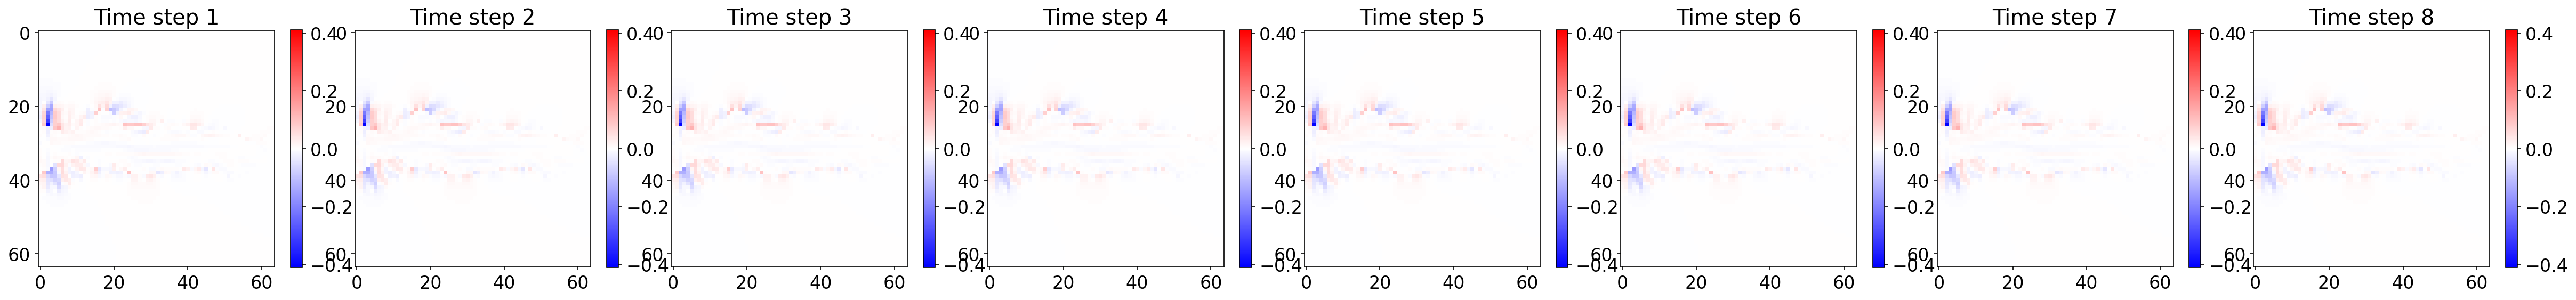
\includegraphics[width=1\textwidth,height=\textheight]{../../plot/GCS_channel_plot/training/JAC_0.5/true_eigvec_1.png}

}

\caption{Static eigenvector}

\end{figure}%%
\begin{figure}[H]

{\centering 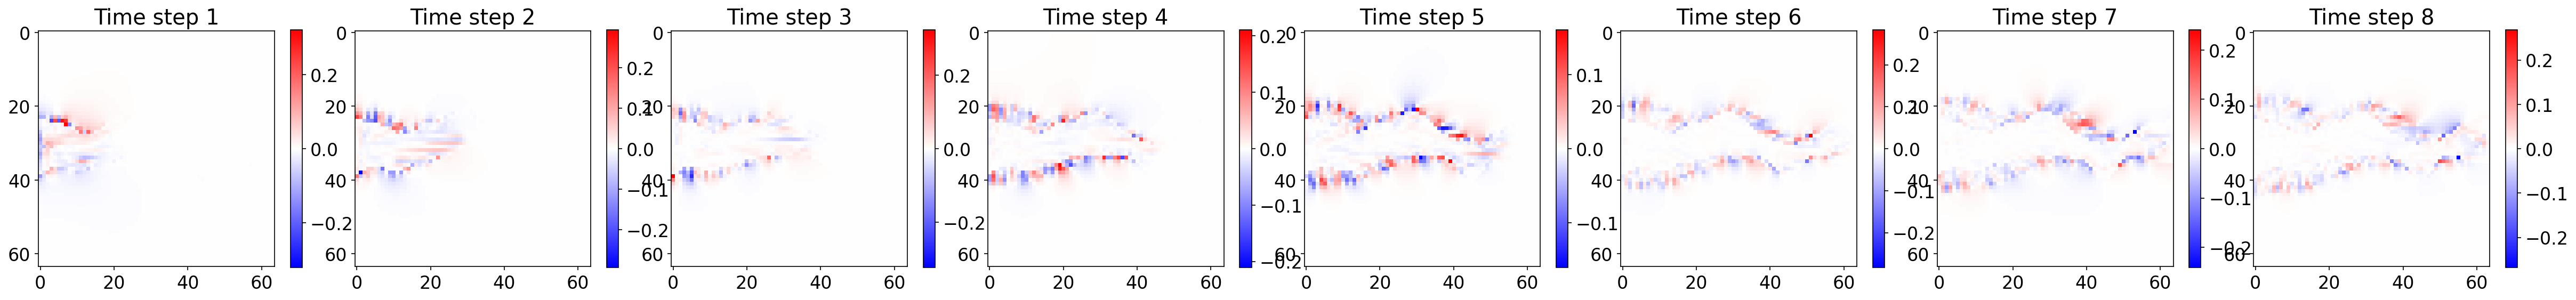
\includegraphics[width=1\textwidth,height=\textheight]{../../plot/GCS_channel_plot/training/JAC/true_eigvec_1.png}

}

\caption{Dynamic eigenvector}

\end{figure}%

\subsection{How does it impact
training?}\label{how-does-it-impact-training}

When we look at the test loss, we observe that unlike static model,
dynamic model's test curve is always lower than that of MSE model.

\begin{figure}

\begin{minipage}{0.50\linewidth}

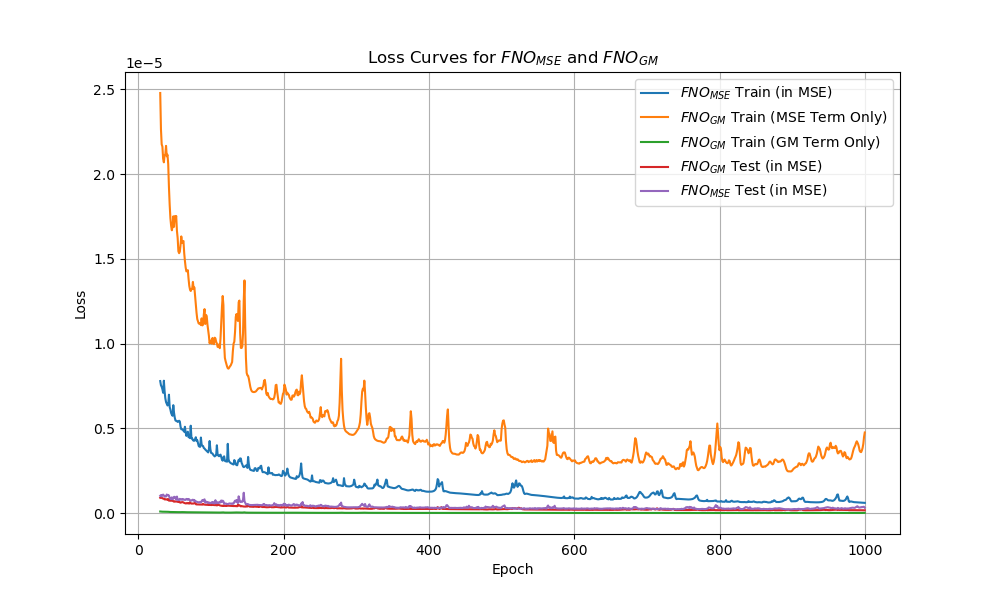
\includegraphics[width=1\textwidth,height=\textheight]{../../test/all_loss_prev_same_eig.png}

\subcaption{\label{}Loss (static)}
\end{minipage}%
%
\begin{minipage}{0.50\linewidth}

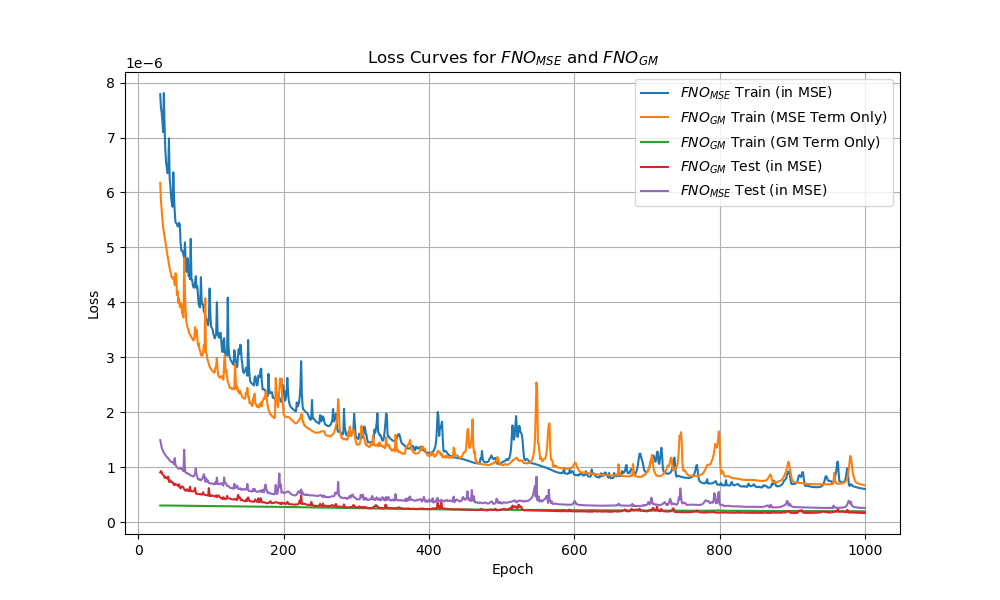
\includegraphics[width=1\textwidth,height=\textheight]{../../test/all_loss.png}

\subcaption{\label{}Loss (dynamic)}
\end{minipage}%

\caption{\label{fig-loss}Loss plot static vs dynamic}

\end{figure}%

\begin{longtable}[]{@{}
  >{\raggedright\arraybackslash}p{(\columnwidth - 8\tabcolsep) * \real{0.1852}}
  >{\raggedright\arraybackslash}p{(\columnwidth - 8\tabcolsep) * \real{0.1111}}
  >{\raggedright\arraybackslash}p{(\columnwidth - 8\tabcolsep) * \real{0.1111}}
  >{\raggedright\arraybackslash}p{(\columnwidth - 8\tabcolsep) * \real{0.2963}}
  >{\raggedright\arraybackslash}p{(\columnwidth - 8\tabcolsep) * \real{0.2963}}@{}}
\toprule\noalign{}
\begin{minipage}[b]{\linewidth}\raggedright
\end{minipage} & \begin{minipage}[b]{\linewidth}\raggedright
Epochs
\end{minipage} & \begin{minipage}[b]{\linewidth}\raggedright
\(\lambda\)
\end{minipage} & \begin{minipage}[b]{\linewidth}\raggedright
Train Loss
\end{minipage} & \begin{minipage}[b]{\linewidth}\raggedright
Test Loss
\end{minipage} \\
\midrule\noalign{}
\endhead
\bottomrule\noalign{}
\endlastfoot
& & & MSE/GM & MSE \\
FNO-MSE & 1000 & N.A. & \(6.5207 \times 10^{-8}\) &
\(1.3088 \times 10^{-7}\) \\
FNO-PBI & 1000 & 1.0 & \(8.3925 \times 10^{-8}\) &
\(1.3030\times 10^{-7}\) \\
\end{longtable}

\subsection{Forward Simulation on Test
dataset}\label{forward-simulation-on-test-dataset}

\begin{figure}

\begin{minipage}{\linewidth}

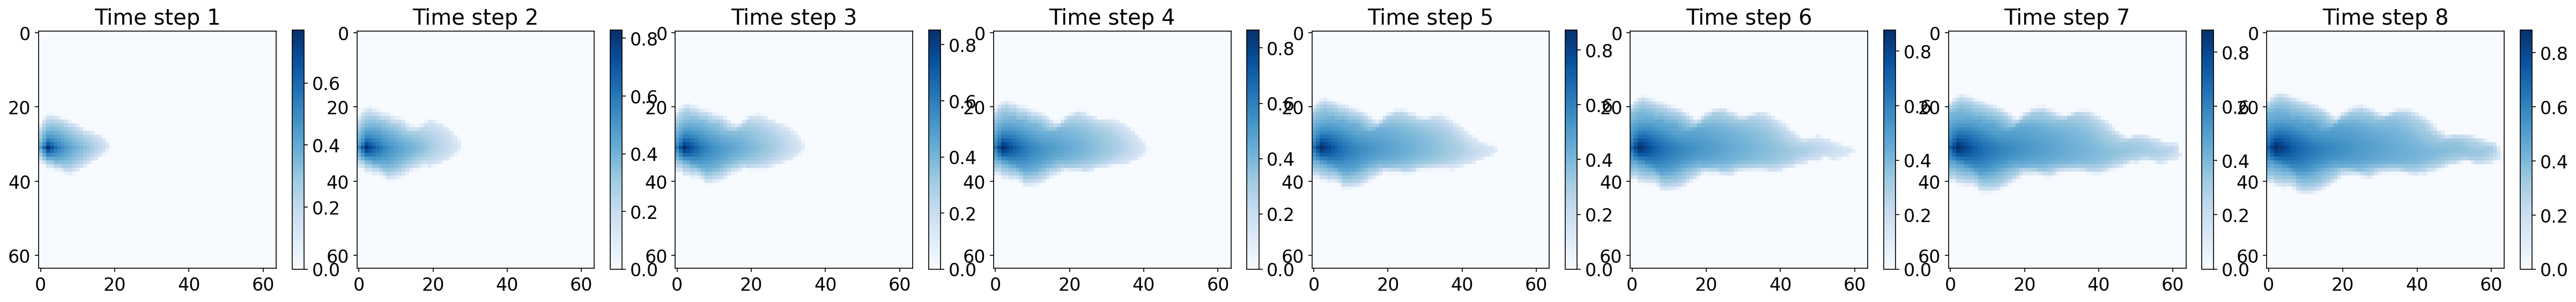
\includegraphics[width=1\textwidth,height=\textheight]{../../plot/GCS_channel_plot/FNO_GCS_lowest_MSE_True.png}

\subcaption{\label{}True Saturation}
\end{minipage}%
\newline
\begin{minipage}{\linewidth}

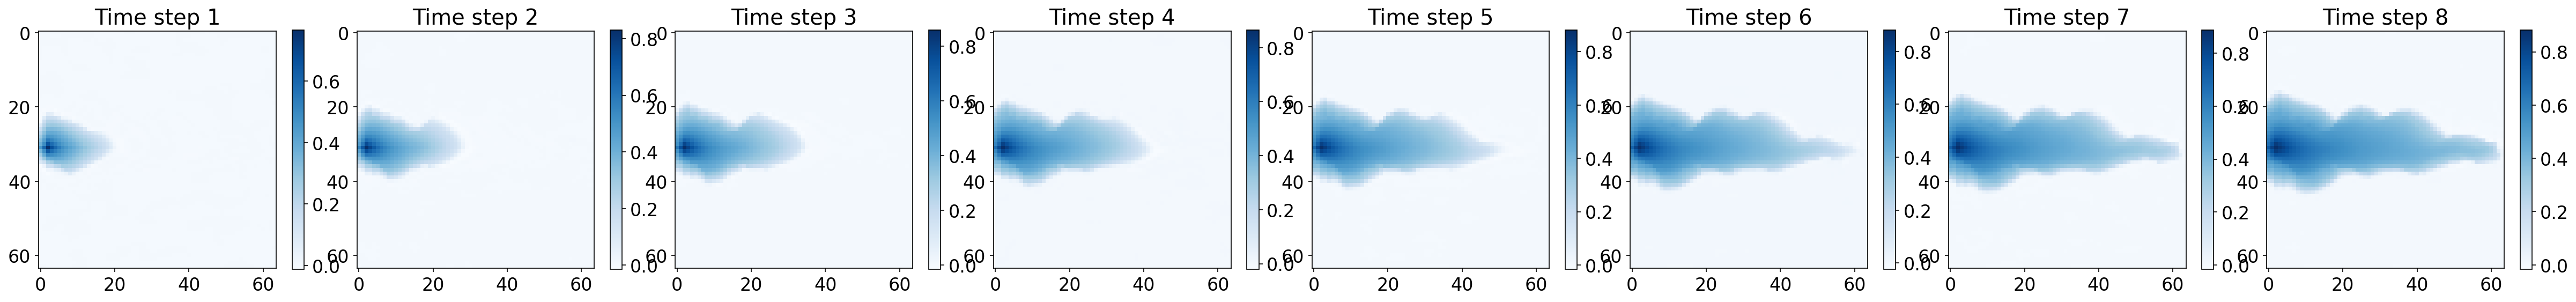
\includegraphics[width=1\textwidth,height=\textheight]{../../plot/GCS_channel_plot/FNO_GCS_lowest_MSE_Pred.png}

\subcaption{\label{}Predicted Saturation: MSE}
\end{minipage}%
\newline
\begin{minipage}{\linewidth}

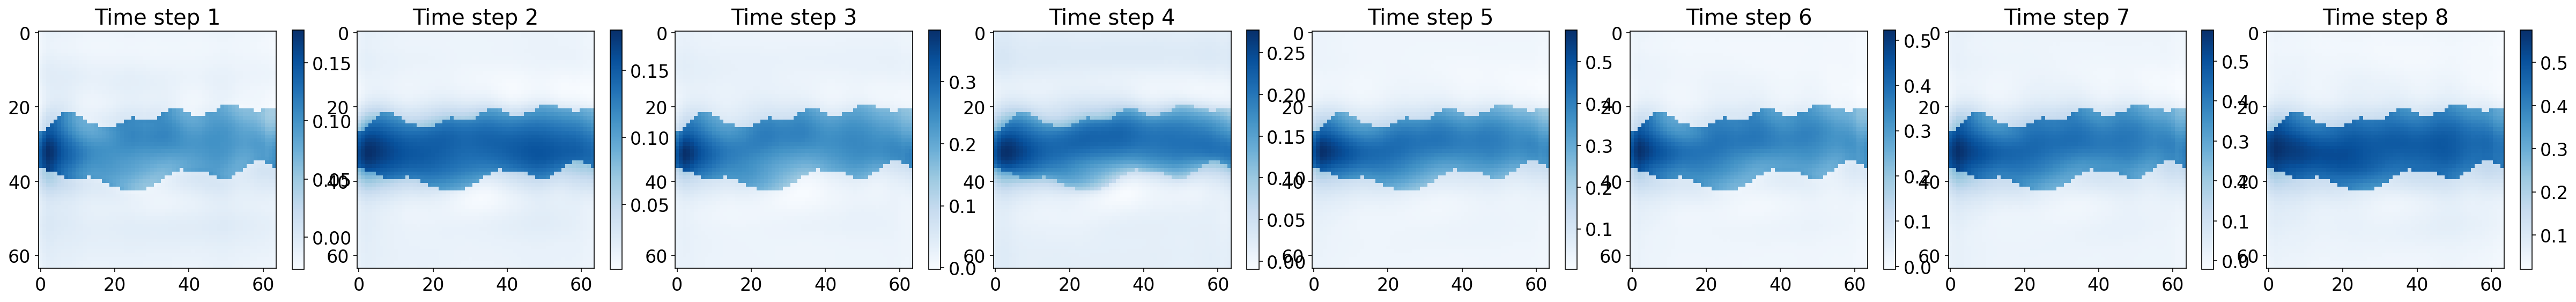
\includegraphics[width=1\textwidth,height=\textheight]{../../plot/GCS_channel_plot/FNO_GCS_lowest_JAC_Pred.png}

\subcaption{\label{}Predicted Saturation: PBI (dynamic)}
\end{minipage}%

\caption{\label{fig-eig1000}Example of Forward Prediction}

\end{figure}%

\begin{figure}

\begin{minipage}{\linewidth}

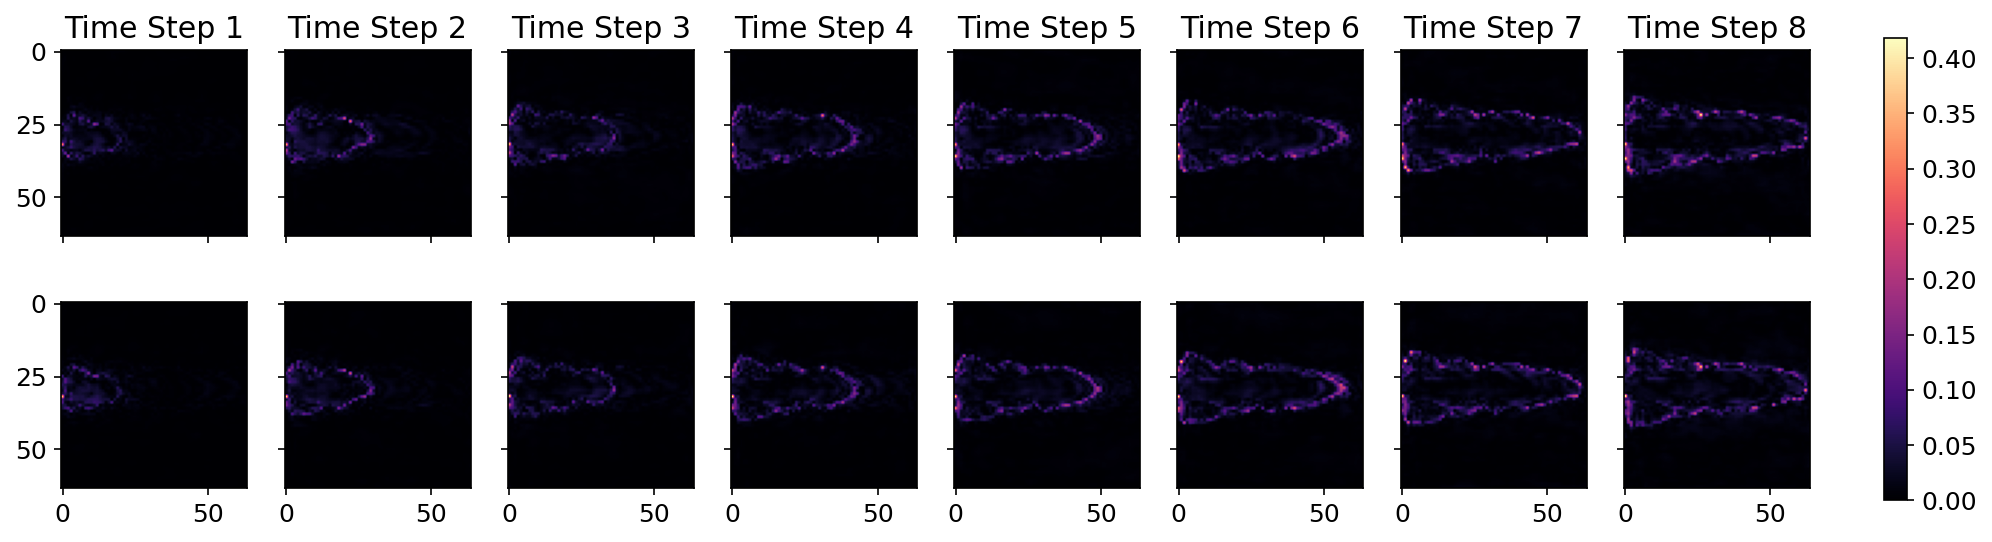
\includegraphics[width=1\textwidth,height=\textheight]{../../gen_sample/GCS_sample/forward_pred_test_diff1.png}

\subcaption{\label{}Test Sample 1}
\end{minipage}%
\newline
\begin{minipage}{\linewidth}

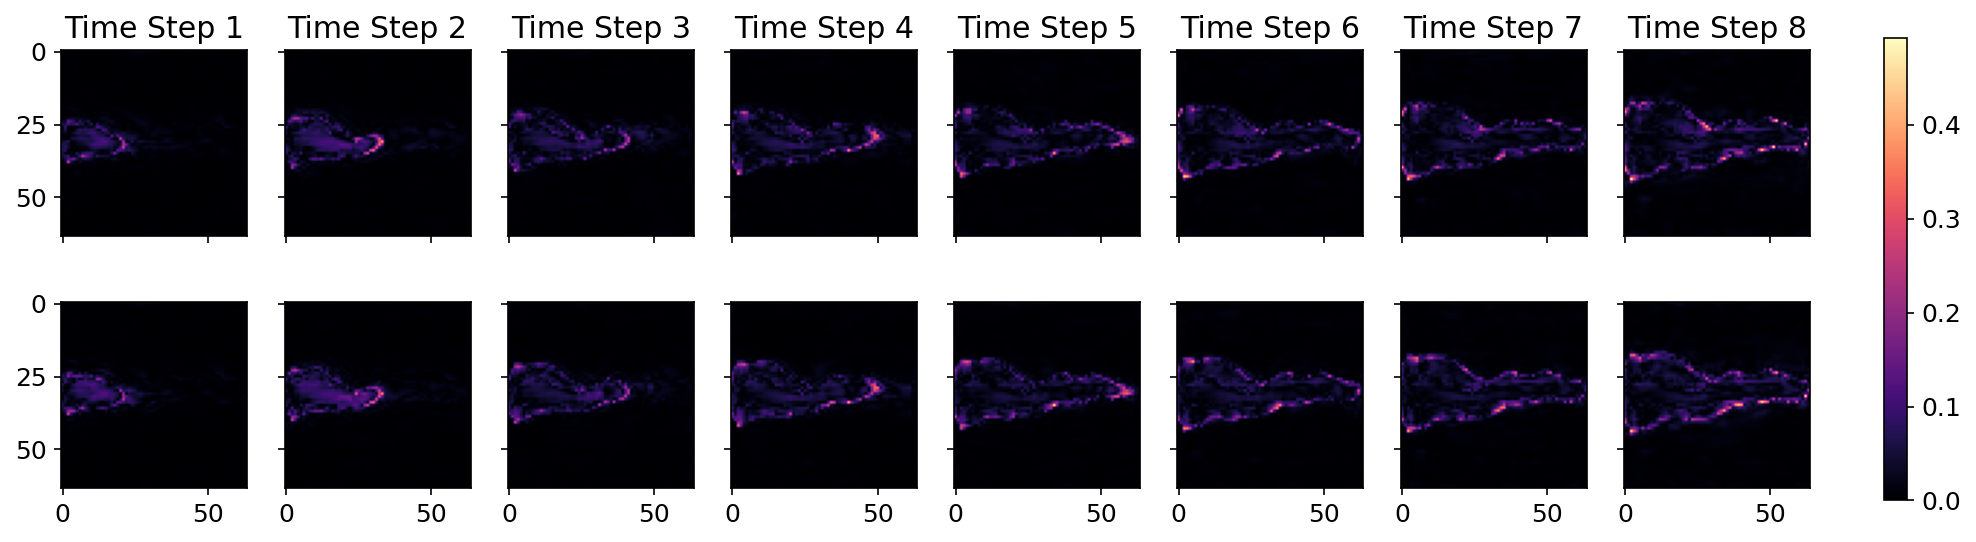
\includegraphics[width=1\textwidth,height=\textheight]{../../gen_sample/GCS_sample/forward_pred_test_diff2.png}

\subcaption{\label{}Test Sample 2}
\end{minipage}%
\newline
\begin{minipage}{\linewidth}

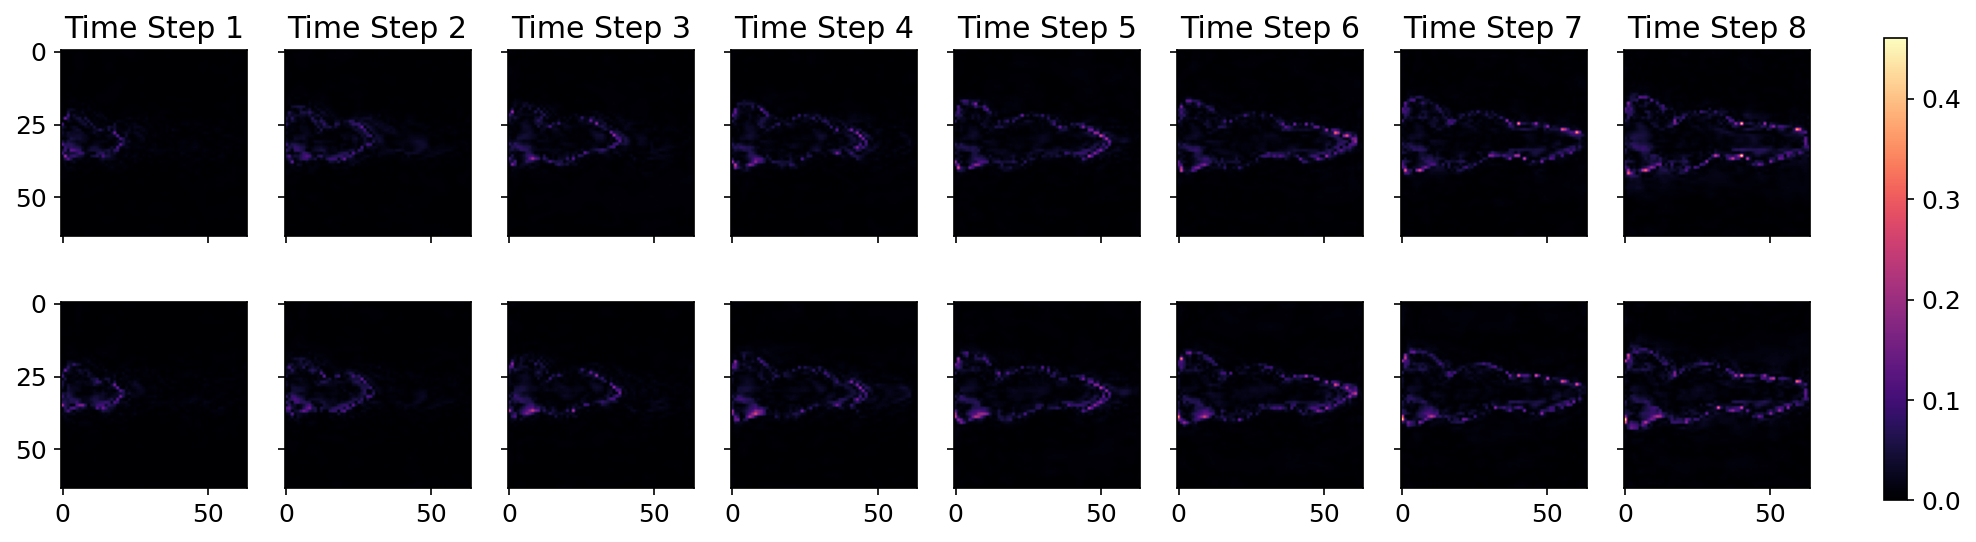
\includegraphics[width=1\textwidth,height=\textheight]{../../gen_sample/GCS_sample/forward_pred_test_diff3.png}

\subcaption{\label{}Test Sample 3}
\end{minipage}%

\caption{\label{fig-eig1000}Absolute Difference (x 5) plot of test
samples}

\end{figure}%

\subsection{Sanity check: how does vJp of MSE model and PBI model look
like?}\label{sanity-check-how-does-vjp-of-mse-model-and-pbi-model-look-like}

\begin{figure}[H]

{\centering 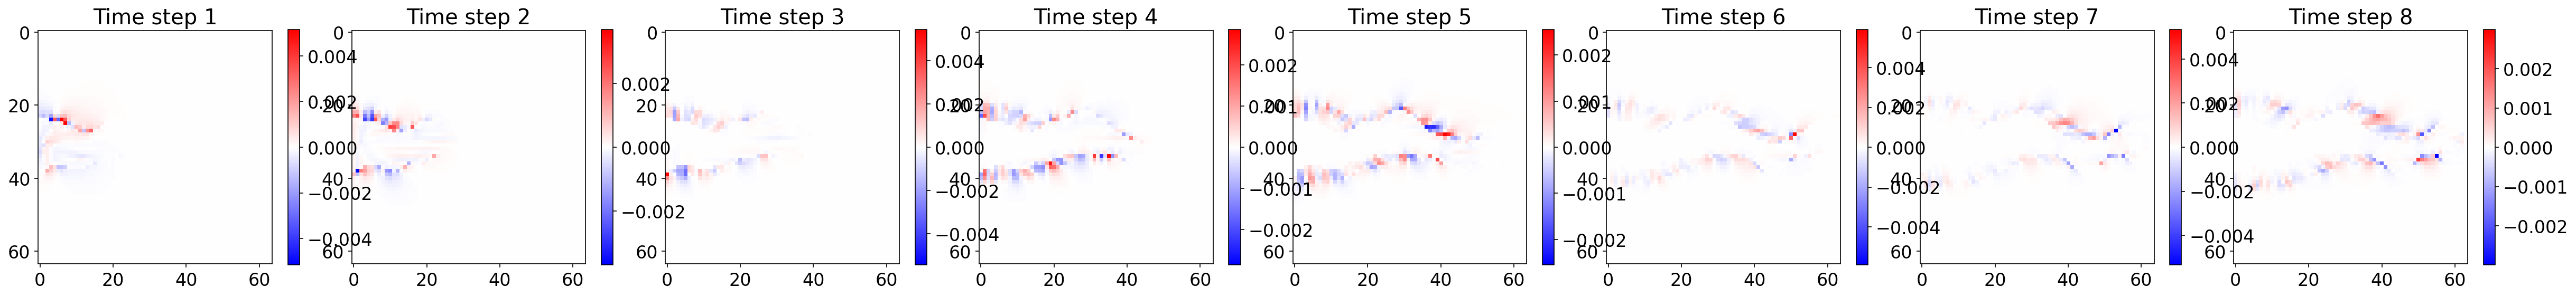
\includegraphics[width=1\textwidth,height=\textheight]{../../plot/GCS_channel_plot/training/JAC/true_vjp_1.png}

}

\caption{Dynamic vJp (True)}

\end{figure}%%
\begin{figure}[H]

{\centering 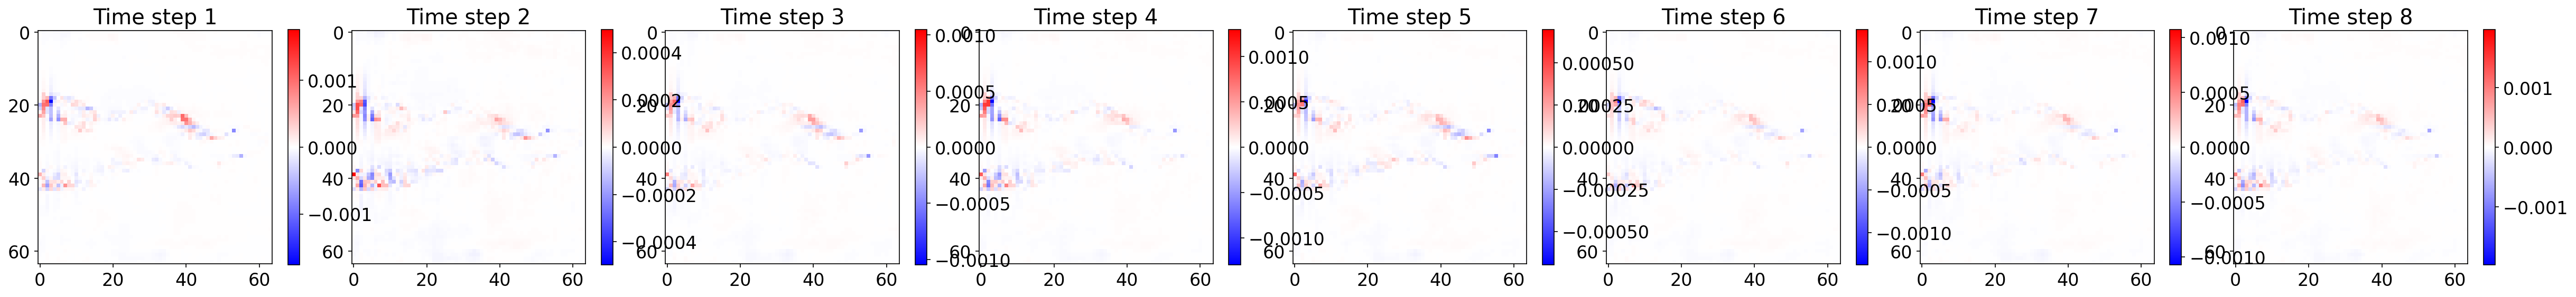
\includegraphics[width=1\textwidth,height=\textheight]{../../plot/GCS_channel_plot/training/MSE/learned_vjp_990.png}

}

\caption{Learned vJp (MSE)}

\end{figure}%%
\begin{figure}[H]

{\centering 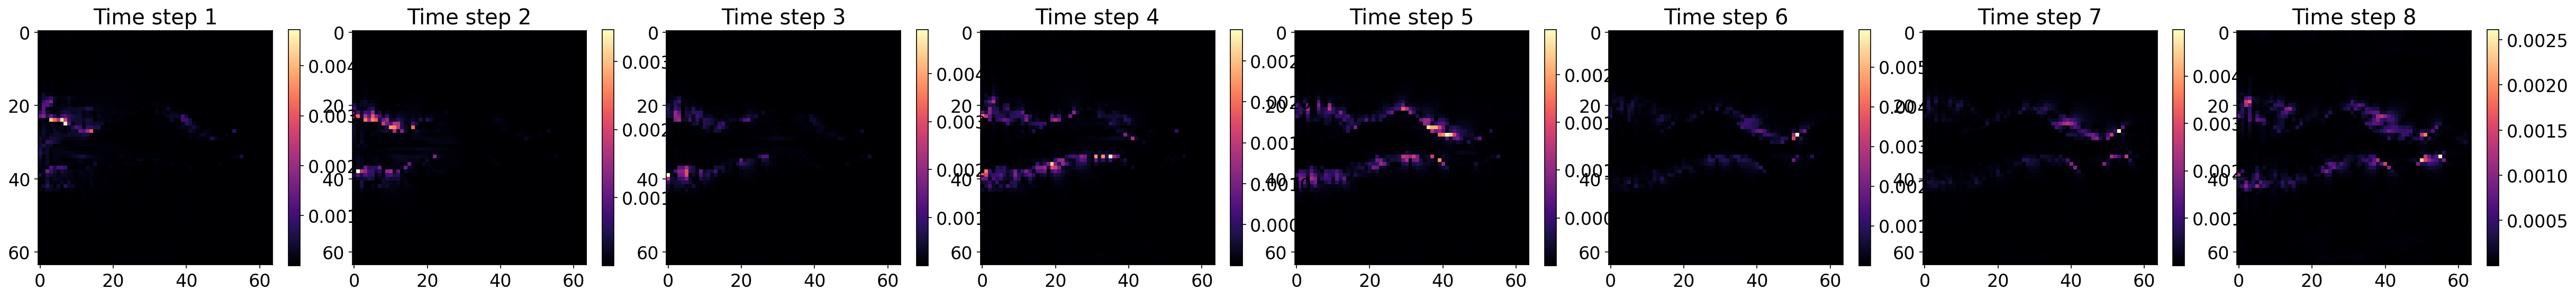
\includegraphics[width=1\textwidth,height=\textheight]{../../plot/GCS_channel_plot/training/MSE/diff_vjp_990.png}

}

\caption{Abs Diff in vJp (MSE)}

\end{figure}%%
\begin{figure}[H]

{\centering 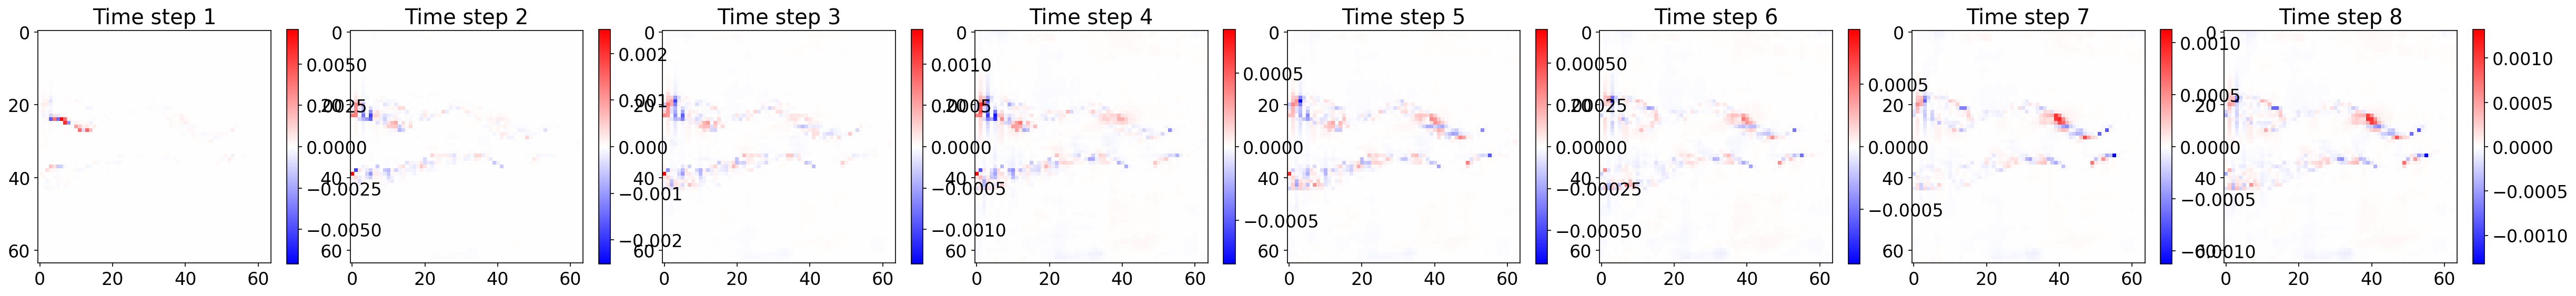
\includegraphics[width=1\textwidth,height=\textheight]{../../plot/GCS_channel_plot/training/JAC/learned_vjp_990.png}

}

\caption{Learned vJp (PBI)}

\end{figure}%%
\begin{figure}[H]

{\centering 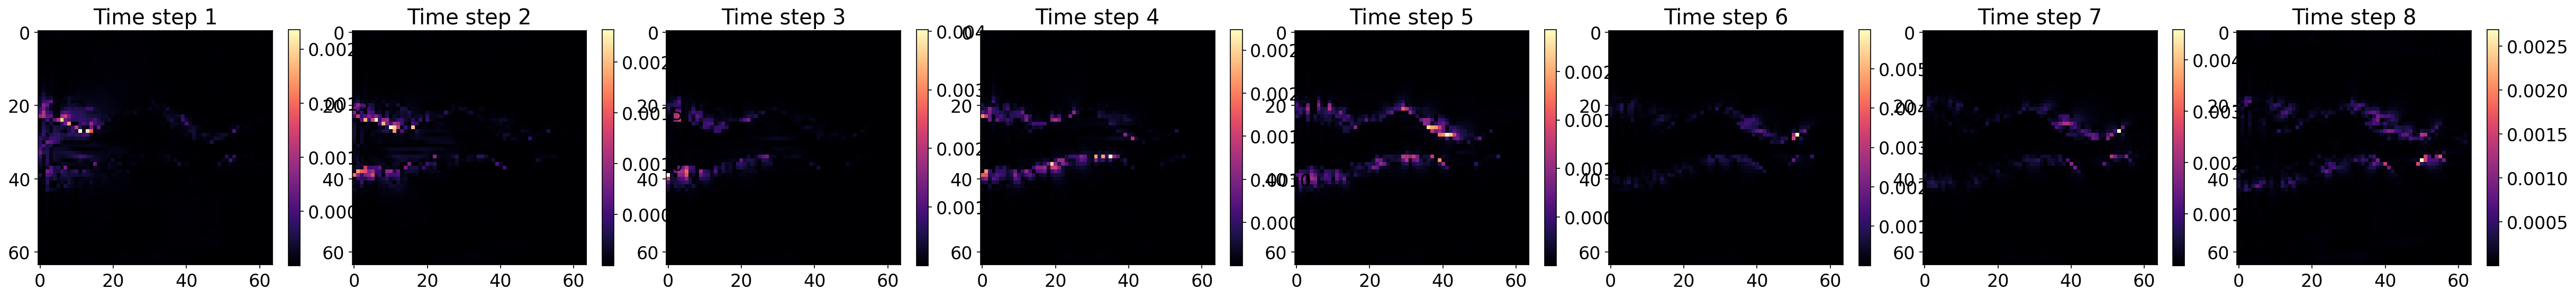
\includegraphics[width=1\textwidth,height=\textheight]{../../plot/GCS_channel_plot/training/JAC/diff_vjp_990.png}

}

\caption{Abs Diff in vJp (PBI)}

\end{figure}%

\section{Inverse}\label{inverse}

Previously, we showed MLE estimate of \(\tilde K\).

\begin{itemize}
\tightlist
\item
  The inversion result looked too good to be true.
\item
  This is because initial \(K_0\) is unperturbed true \(K\), so there
  was nothing to optimize upon.
\item
  So now we perturbed \(K_0\) like Francis did.
\end{itemize}

\subsection{Setting}\label{setting}

We wanted to evaluate surrogate model's performace in MLE/posterior
estimation quickly, so for now, we kept inversion method as simple as
possible. (least squares method)

\begin{quote}
\(min_{K} \|S_{\theta}(K) - S(K)\|_2^2\)

where:

\begin{itemize}
\tightlist
\item
  \(K_0\) = \(H(K)\)
\item
  \(S_{\theta}\): Neural Network model
\end{itemize}
\end{quote}

\hfill\break

\begin{itemize}
\tightlist
\item
  We obtain 100 \(\{S^t(K)\}_{t=1}^8\) from test data.
\item
  We generate \(H(K_0)\) by averaging over all \(K_0\) where \(H\) is
  observation operator.
\end{itemize}

Now we look at two different cases:

\begin{enumerate}
\def\labelenumi{\arabic{enumi}.}
\tightlist
\item
  static
\item
  dynamic
\end{enumerate}

\subsection{Loss}\label{loss}

With dynamic eigenvector, the loss during inversion falls under that of
MSE model.

\begin{figure}[H]

{\centering 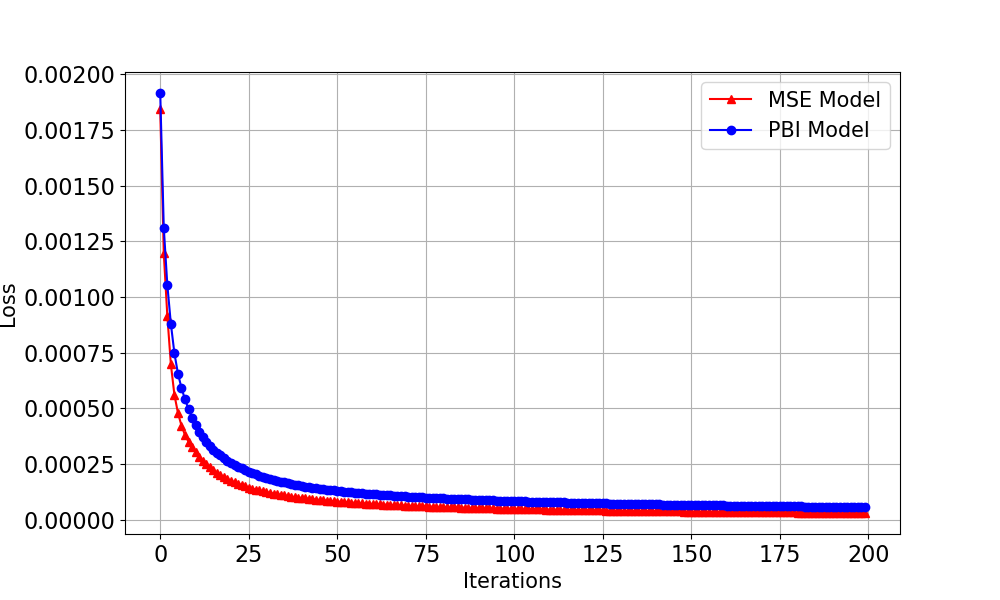
\includegraphics[width=1\textwidth,height=\textheight]{../../gen_sample/GCS_partial/both_0/loss_plot_100.0_200_same_eig.png}

}

\caption{Loss (static)}

\end{figure}%%
\begin{figure}[H]

{\centering 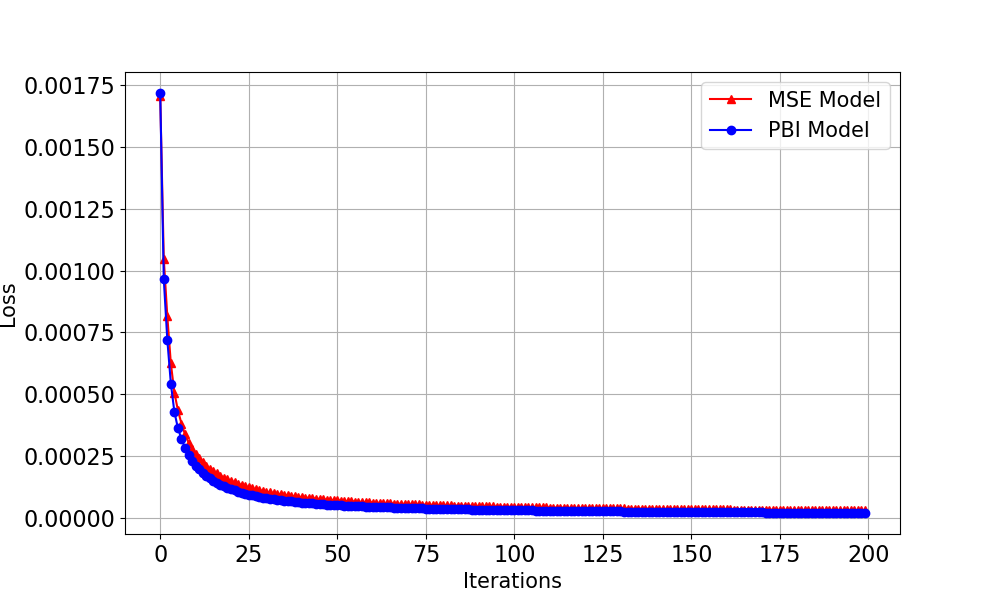
\includegraphics[width=1\textwidth,height=\textheight]{../../gen_sample/GCS_partial/both_0/loss_plot_100.0_200.png}

}

\caption{Loss (dynamic)}

\end{figure}%

\subsection{Ablation test: finding optimal lambda and number of
epoch}\label{ablation-test-finding-optimal-lambda-and-number-of-epoch}

\subsubsection{Choosing the best parameters for MLE
optimization}\label{choosing-the-best-parameters-for-mle-optimization}

We conduct hyperparameter search for the \(\lambda\). The number of
epochs chosen were based on the loss plot convergence. If it converged,
we stopped training.

This is unconstrained.

\paragraph{Unconstrained (static)}\label{unconstrained-static}

\begin{longtable}[]{@{}
  >{\raggedright\arraybackslash}p{(\columnwidth - 8\tabcolsep) * \real{0.2055}}
  >{\raggedright\arraybackslash}p{(\columnwidth - 8\tabcolsep) * \real{0.1233}}
  >{\raggedright\arraybackslash}p{(\columnwidth - 8\tabcolsep) * \real{0.1233}}
  >{\raggedright\arraybackslash}p{(\columnwidth - 8\tabcolsep) * \real{0.3288}}
  >{\raggedright\arraybackslash}p{(\columnwidth - 8\tabcolsep) * \real{0.2192}}@{}}
\toprule\noalign{}
\begin{minipage}[b]{\linewidth}\raggedright
\end{minipage} & \begin{minipage}[b]{\linewidth}\raggedright
Epochs
\end{minipage} & \begin{minipage}[b]{\linewidth}\raggedright
\(\lambda\)
\end{minipage} & \begin{minipage}[b]{\linewidth}\raggedright
Loss (MSE)
\end{minipage} & \begin{minipage}[b]{\linewidth}\raggedright
SSIM
\end{minipage} \\
\midrule\noalign{}
\endhead
\bottomrule\noalign{}
\endlastfoot
FNO-PBI & 400 & 20.0 & \(8.9021 \times 10^{-5}\) & \(0.5550\) \\
FNO-PBI & 300 & 50.0 & \(6.1867 \times 10^{-5}\) & \(0.5555\) \\
FNO-PBI & 200 & 100.0 & \(5.5757 \times 10^{-5}\) & \(0.5709\) \\
--------------- & --------- & --------- & ------------------------ &
---------------- \\
FNO-MSE & 400 & 20.0 & \(5.3901 \times 10^{-5}\) & \(0.5235\) \\
FNO-MSE & 300 & 50.0 & \(3.4602 \times 10^{-5}\) & \(0.5428\) \\
FNO-MSE & 200 & 100.0 & \(2.9429 \times 10^{-5}\) & \(0.5564\) \\
\end{longtable}

\subsubsection{Updated Result}\label{updated-result}

Out of all 100 test samples, I brought some interesting cases. Some
looks good, some looks questionable. (Test sample 3, 5). Does SSIM
values make sense here?

\begin{figure}[H]

{\centering \includegraphics[width=1\textwidth,height=\textheight]{../../gen_sample/GCS_partial/both_0_100.0_same_eig/posterior_199_0_84.png}

}

\caption{Test sample 1 (static)}

\end{figure}%%
\begin{figure}[H]

{\centering \includegraphics[width=1\textwidth,height=\textheight]{../../gen_sample/GCS_partial/both_0_100.0_same_eig/posterior_199_0_67.png}

}

\caption{Test sample 2 (static)}

\end{figure}%%
\begin{figure}[H]

{\centering \includegraphics[width=1\textwidth,height=\textheight]{../../gen_sample/GCS_partial/both_0_100.0_same_eig/posterior_199_0_89.png}

}

\caption{Test sample 3 (static)}

\end{figure}%%
\begin{figure}[H]

{\centering \includegraphics[width=1\textwidth,height=\textheight]{../../gen_sample/GCS_partial/both_0_100.0_same_eig/posterior_199_0_85.png}

}

\caption{Test sample 4 (static)}

\end{figure}%%
\begin{figure}[H]

{\centering \includegraphics[width=1\textwidth,height=\textheight]{../../gen_sample/GCS_partial/both_0_100.0_same_eig/posterior_199_0_90.png}

}

\caption{Test sample 5 (static)}

\end{figure}%

\subsubsection{What other things can be evaluated in terms of forward
simulation?}\label{what-other-things-can-be-evaluated-in-terms-of-forward-simulation}

\begin{enumerate}
\def\labelenumi{\arabic{enumi}.}
\tightlist
\item
  \textbf{Stability}: predict longer saturation evolution 9th to 16th.
\item
  \textbf{Generalization}: test with out of distribution test samples.
\item
  \textbf{Towards learning true governing PDE equation}: One step
  prediction rather than multi-step prediction
\end{enumerate}

\begin{itemize}
\tightlist
\item
  Current one is time discretized.
\end{itemize}

\section{Conclusion}\label{conclusion}

\begin{itemize}
\tightlist
\item
  As of right now, we don't see significant difference between MSE and
  PBI model in terms of posterior estimate.

  \begin{itemize}
  \tightlist
  \item
    It is likely undertrained.
  \end{itemize}
\end{itemize}

\section{Updates:}\label{updates}

\begin{itemize}
\tightlist
\item
  To train FNO with multiple eigenvectors, have been generating dataset.
  For 1000 data points, we are obtaining the first 20 eigenvectors.
\item
  However, number of observation is 20 (before it was 2) to get the FIM
  and we call Zygote.pullback 20 times per sample to get vJp, so it
  takes some time.
\item
  We also had some debugged some code issues.
\item
  So right now, tested with

  \begin{itemize}
  \tightlist
  \item
    100 training sample,
  \item
    50 test samples
  \item
    500 epochs.
  \end{itemize}
\item
  And we show preliminary results with 3 different scenarios: when
  number of vector is 1, 3, 5.
\end{itemize}

\subsection{Forward Simulation on Test
Dataset}\label{forward-simulation-on-test-dataset-1}

\begin{longtable}[]{@{}
  >{\raggedright\arraybackslash}p{(\columnwidth - 8\tabcolsep) * \real{0.1807}}
  >{\raggedright\arraybackslash}p{(\columnwidth - 8\tabcolsep) * \real{0.1325}}
  >{\raggedright\arraybackslash}p{(\columnwidth - 8\tabcolsep) * \real{0.1084}}
  >{\raggedright\arraybackslash}p{(\columnwidth - 8\tabcolsep) * \real{0.2892}}
  >{\raggedright\arraybackslash}p{(\columnwidth - 8\tabcolsep) * \real{0.2892}}@{}}
\toprule\noalign{}
\begin{minipage}[b]{\linewidth}\raggedright
\end{minipage} & \begin{minipage}[b]{\linewidth}\raggedright
number of \(\vec{x}\)
\end{minipage} & \begin{minipage}[b]{\linewidth}\raggedright
\(\lambda\)
\end{minipage} & \begin{minipage}[b]{\linewidth}\raggedright
Train Loss
\end{minipage} & \begin{minipage}[b]{\linewidth}\raggedright
Test Loss
\end{minipage} \\
\midrule\noalign{}
\endhead
\bottomrule\noalign{}
\endlastfoot
& & & MSE/GM & MSE \\
FNO-MSE & N.A. & N.A. & \(2.0915 \times 10^{-7}\) &
\(8.08192 \times 10^{-7}\) \\
FNO-PBI & 1 & 0.65 & \(3.8140 \times 10^{-7}\) &
\(8.0472\times 10^{-7}\) \\
FNO-PBI & 3 & 0.65 & \(3.0985 \times 10^{-7}\) &
\(8.2933\times 10^{-7}\) \\
FNO-PBI & 5 & 0.65 & \(2.6275 \times 10^{-7}\) &
\(8.2738\times 10^{-7}\) \\
\end{longtable}

\begin{figure}

\begin{minipage}{\linewidth}

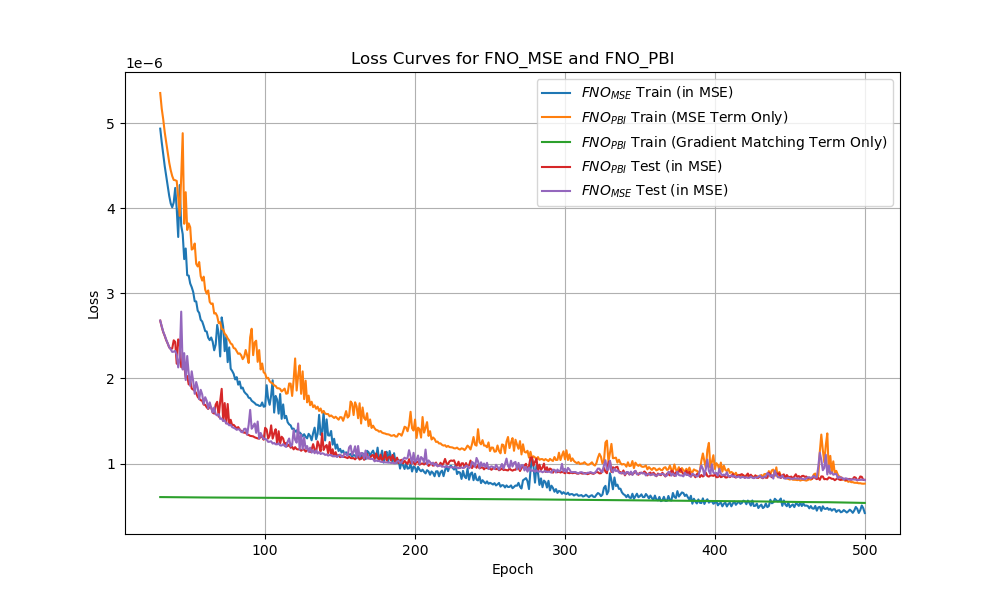
\includegraphics[width=1\textwidth,height=\textheight]{../../test/all_loss_1.png}

\subcaption{\label{}All}
\end{minipage}%
\newline
\begin{minipage}{\linewidth}

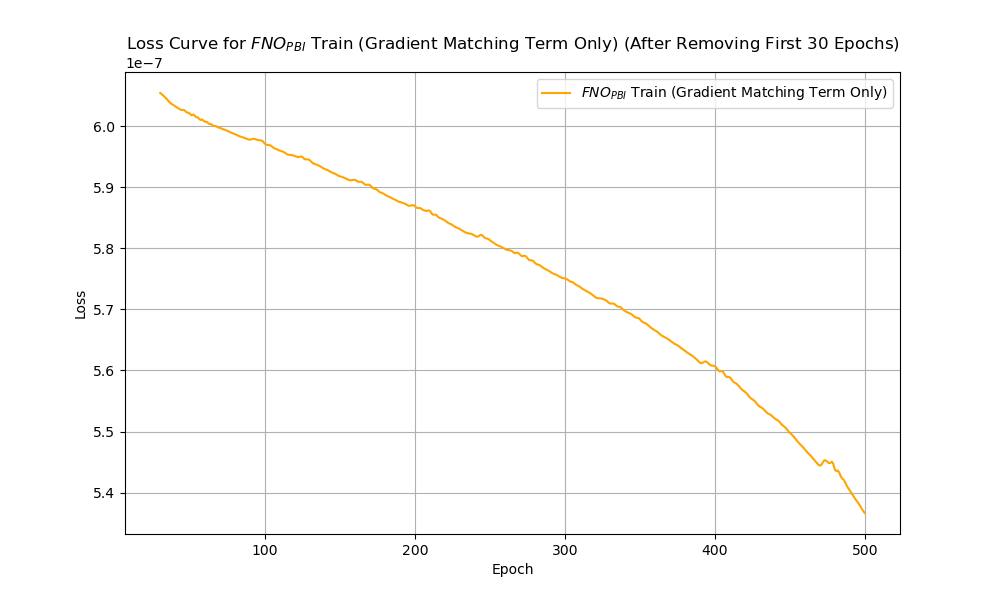
\includegraphics[width=1\textwidth,height=\textheight]{../../test/PBI_term_1.png}

\subcaption{\label{}GM term}
\end{minipage}%

\caption{\label{fig-eig1000}When number of eigenvector = 1}

\end{figure}%

\begin{figure}

\begin{minipage}{\linewidth}

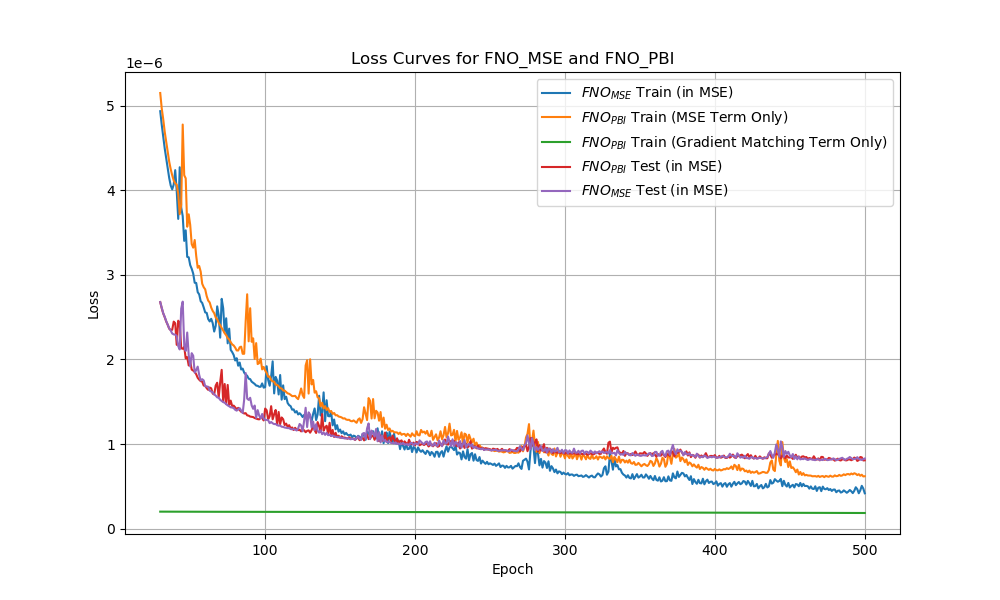
\includegraphics[width=1\textwidth,height=\textheight]{../../test/all_loss_3.png}

\subcaption{\label{}All}
\end{minipage}%
\newline
\begin{minipage}{\linewidth}

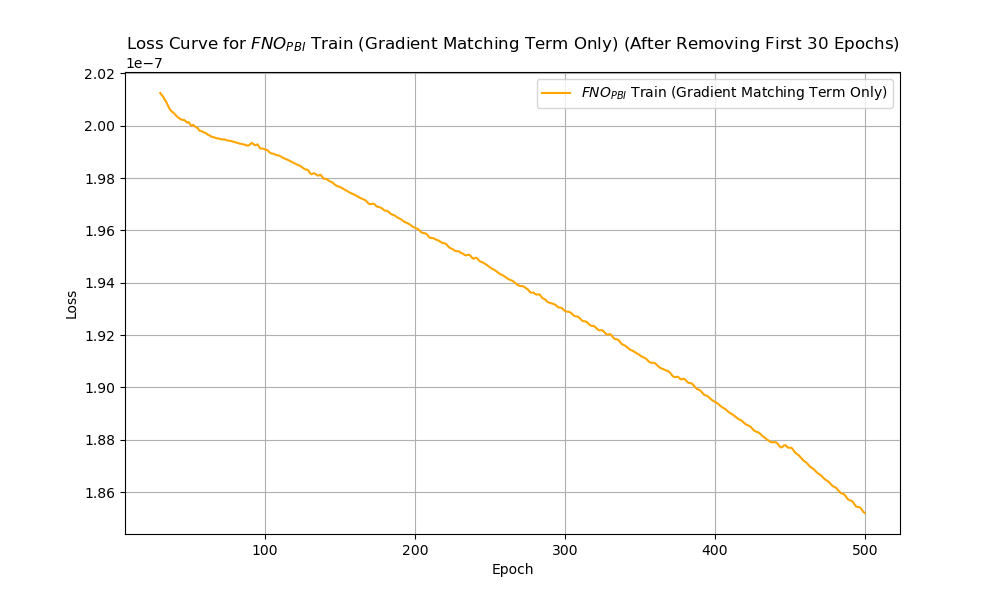
\includegraphics[width=1\textwidth,height=\textheight]{../../test/PBI_term_3.png}

\subcaption{\label{}GM term}
\end{minipage}%

\caption{\label{fig-eig1000}When number of eigenvector = 3}

\end{figure}%

\begin{figure}

\begin{minipage}{\linewidth}

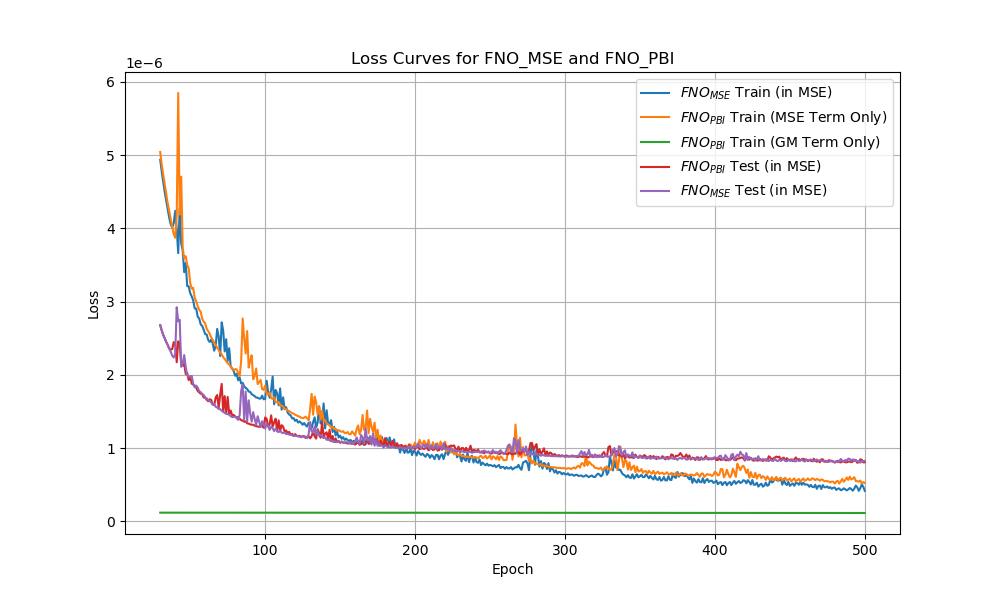
\includegraphics[width=1\textwidth,height=\textheight]{../../test/all_loss_5.png}

\subcaption{\label{}All}
\end{minipage}%
\newline
\begin{minipage}{\linewidth}

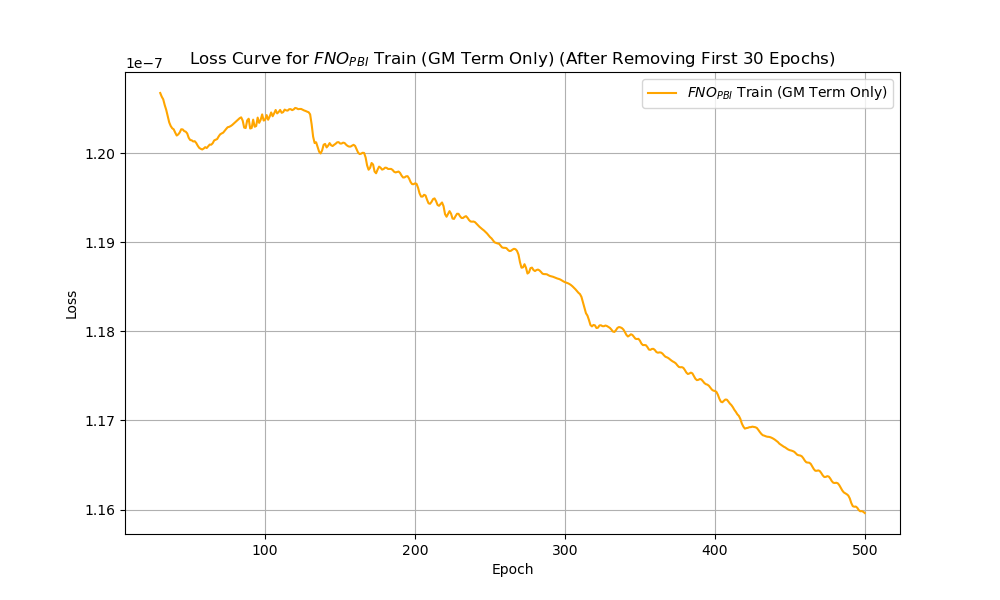
\includegraphics[width=1\textwidth,height=\textheight]{../../test/PBI_term_5.png}

\subcaption{\label{}GM term}
\end{minipage}%

\caption{\label{fig-eig1000}When number of eigenvector = 5}

\end{figure}%

\subsection{MLE Estimate vs Number of
Eigenvector}\label{mle-estimate-vs-number-of-eigenvector}

\begin{longtable}[]{@{}
  >{\raggedright\arraybackslash}p{(\columnwidth - 8\tabcolsep) * \real{0.1807}}
  >{\raggedright\arraybackslash}p{(\columnwidth - 8\tabcolsep) * \real{0.1325}}
  >{\raggedright\arraybackslash}p{(\columnwidth - 8\tabcolsep) * \real{0.1084}}
  >{\raggedright\arraybackslash}p{(\columnwidth - 8\tabcolsep) * \real{0.2892}}
  >{\raggedright\arraybackslash}p{(\columnwidth - 8\tabcolsep) * \real{0.2892}}@{}}
\toprule\noalign{}
\begin{minipage}[b]{\linewidth}\raggedright
\end{minipage} & \begin{minipage}[b]{\linewidth}\raggedright
number of \(\vec{x}\)
\end{minipage} & \begin{minipage}[b]{\linewidth}\raggedright
SSIM
\end{minipage} & \begin{minipage}[b]{\linewidth}\raggedright
Forward Loss
\end{minipage} & \begin{minipage}[b]{\linewidth}\raggedright
MSE
\end{minipage} \\
\midrule\noalign{}
\endhead
\bottomrule\noalign{}
\endlastfoot
FNO-MSE & N.A. & \(0.7644\) & \(4.9598 \times 10^{-5}\) & 698.5997 \\
FNO-PBI & 1 & \(0.7667\) & \(4.6305 \times 10^{-5}\) & \(667.3286\) \\
FNO-PBI & 3 & \(0.7670\) & \(4.7811 \times 10^{-5}\) & \(676.3323\) \\
FNO-PBI & 5 & \(0.7650\) & \(4.7420 \times 10^{-5}\) & \(684.8894\) \\
\end{longtable}

\subsection{Some comments on these mediocre
results}\label{some-comments-on-these-mediocre-results}

\begin{enumerate}
\def\labelenumi{\arabic{enumi}.}
\tightlist
\item
\end{enumerate}

\subsection{Side note: testing with one step
prediction}\label{side-note-testing-with-one-step-prediction}

\subsection{Other comment}\label{other-comment}

Will try to finish draft for ML4seismic presentation by Saturday.

\subsection{Future Step}\label{future-step}

\begin{enumerate}
\def\labelenumi{\arabic{enumi}.}
\tightlist
\item
  TODO: Debug NS eigenvector and vjp.
\item
  TODO: Want to generate the full dataset for Francis' dataset (which
  might take 1 or 2 days).
\item
  TODO: Try it on Jason's dataset (Now that we fixed the problem with
  FIM computation, we are optimistic about the experiment, so we want to
  try it again.)
\end{enumerate}




\end{document}
